\documentclass[a4paper,10pt]{article}
\usepackage[T1]{fontenc}
\usepackage[utf8]{inputenc}
\usepackage{lmodern}
\usepackage[sort, numbers]{natbib}
\usepackage{graphicx}
\usepackage{amsmath}


\title{Temperature and energy measurements in ultra-low temperature Helium-3}
\author{PF}

\begin{document}

\maketitle
%\tableofcontents

%\begin{abstract}
%\end{abstract}

%\section{}

Specific heat capacity $C_V$ as a function of the temperature $T$ (in units of [J/K/m$^3$]) has been calculated from the entropy of a system of independent fermions, quasiparticles~\cite{vollhardt}, as

\begin{equation}
C_V(T)=2(2\pi)^{1/2}k_BN(0)\Delta\left(\frac{\Delta}{k_BT}\right)\exp\left(-\frac{\Delta}{k_BT}\right)
\end{equation}

where $k_B$ is the Boltzmann constant, $N(0)$ is the density of quasiparticle states in the normal phase at Fermi energy for one spin component, $\Delta$ ($\approx 1.76 k_B T_c$) is the average gap energy at low temperature near the critical temperature for superfluidity $T_c$ ($\simeq$930\,$\mu$K).

$C_V(T)$ has a strong dependency with temperature (fig.~\ref{fig:CvT})

\begin{figure}[htb]
  \begin{center}
    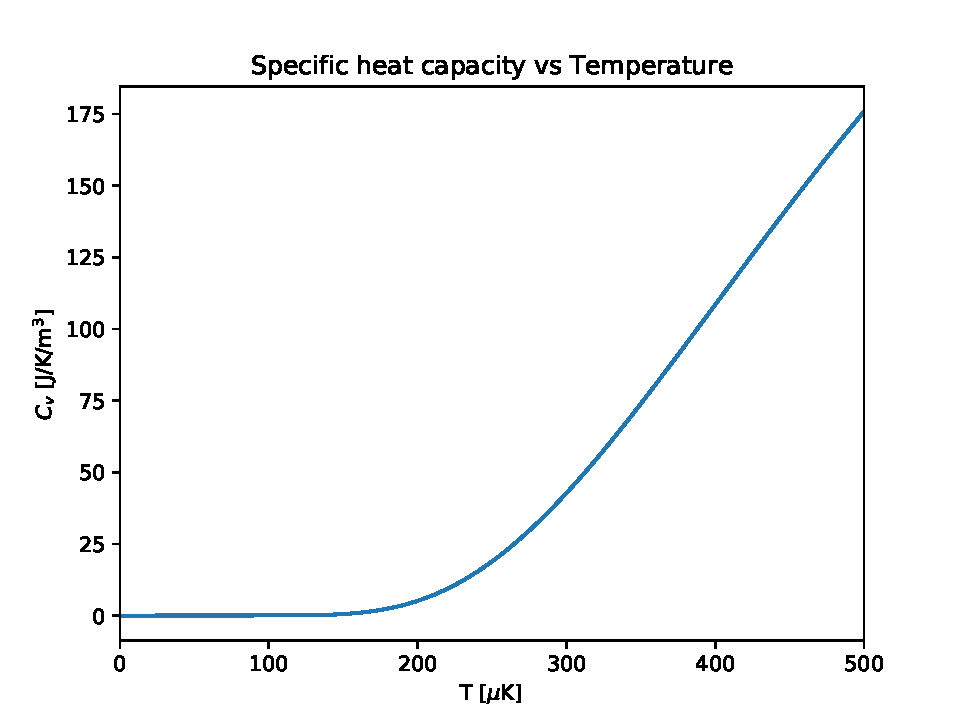
\includegraphics[width=0.69\textwidth]{Cv_vs_T-zoom}
  \end{center}
  \caption{$C_V$ vs T, below $T_c$. He3 has an extremely low heat capacity at low temperatures.}
  \label{fig:CvT}
\end{figure}

To obtain the heat variation $\Delta Q$ between two temperatures $T_1$ and $T_2$ for a a given volume $V$ of helium-3 is required the integration

\begin{align}
\Delta Q (T_1,T_2) = \Delta C_V V & = V \int_{T_1}^{T_2} C_V(T)dT \\
                                  & = V \left( \int_{0}^{T_2} C_V(T)dT - \int_{0}^{T_1} C_V(T)dT \right)\\
                                  & = V \left( I(T_2) - I(T_1) \right)  
\end{align}

where

\begin{align}
I(T) = \int_{0}^{T} C_V(T)dT & = \sqrt{2} \pi N(0) \Delta^2 \left( 1 - \frac{2}{\sqrt{\pi}}\int_{0}^{\sqrt \frac{\Delta}{k_BT}} e^{-t^2} dt \right) \\ 
                             & =  \sqrt{2}\pi N(0)\Delta^2 \mathrm{erfc} \sqrt{\frac{\Delta}{k_BT} } 
\end{align}

therefore

\begin{equation}
\Delta Q (T_1,T_2) = \sqrt{2}\pi N(0)\Delta^2 \left( \mathrm{erfc}\sqrt{\frac{\Delta}{k_BT_2}} - \mathrm{erfc}\sqrt{\frac{\Delta}{k_BT_1}} \right)V
\end{equation}

We consider the 1\,cm$^3$ volume of helium-3 at a certain base temperature $T_0$ so we can calculate the temperature variation $\Delta T$ for an energy deposition $\Delta Q(T_0,T_0+\Delta T)$;
since both $N(0)$ and $\Delta$ are function of the pressure we calculate the energy deposition for 4 different pressures in the range (0--30)\,bar (fig.~\ref{fig:TDE})

\begin{figure}[!ht]
  \begin{center}
  \begin{tabular}{cc}
    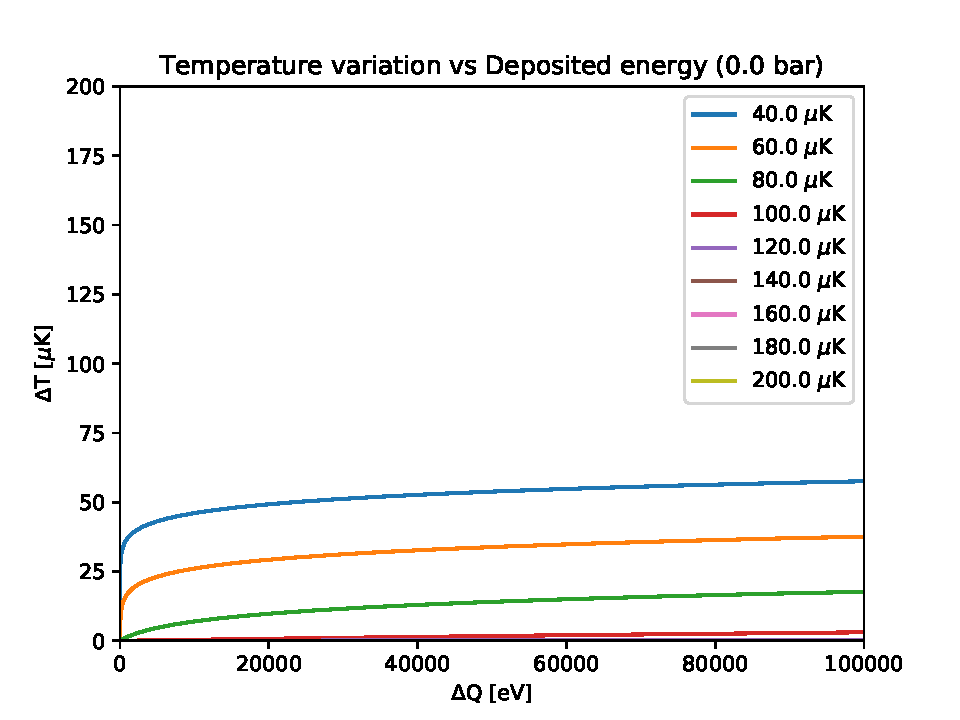
\includegraphics[width=0.49\textwidth]{T_vs_DE-0bar} &
    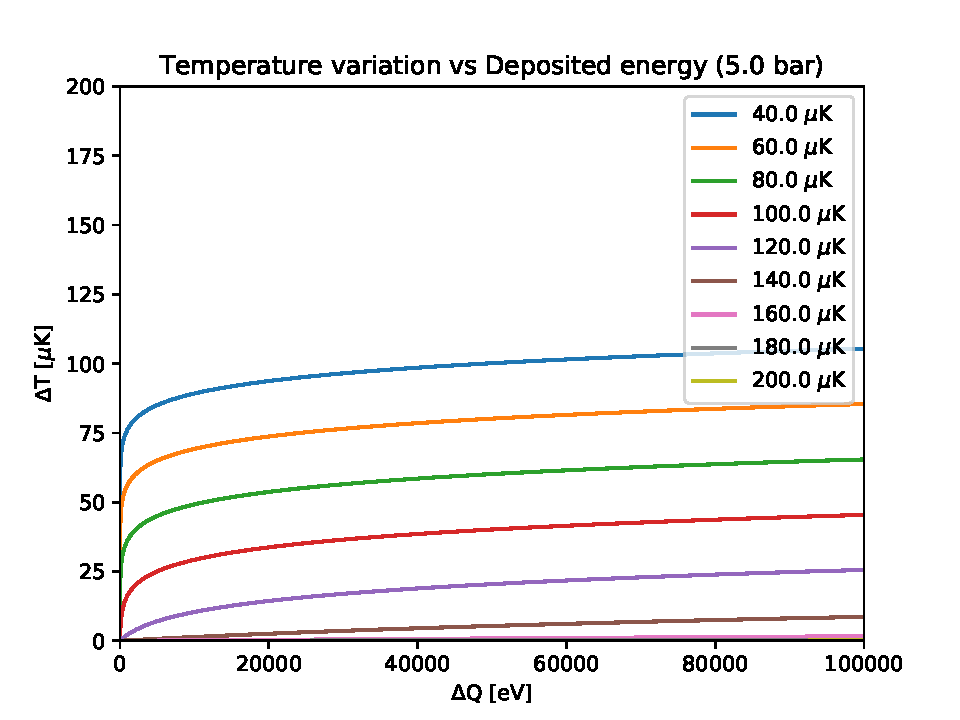
\includegraphics[width=0.49\textwidth]{T_vs_DE-5bar} \\
    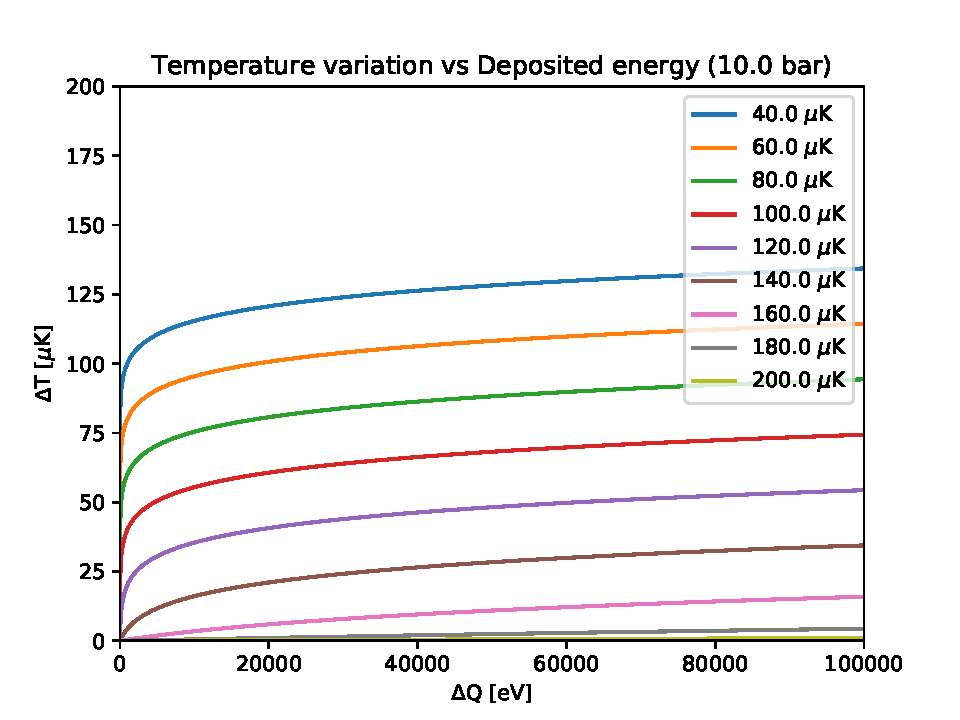
\includegraphics[width=0.49\textwidth]{T_vs_DE-10bar} &
    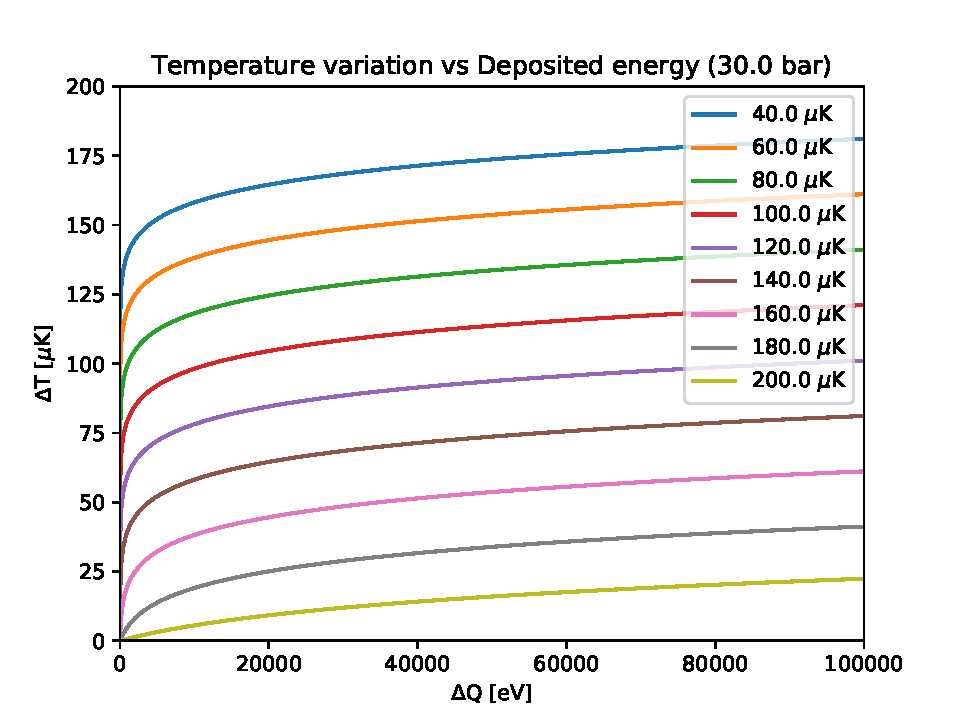
\includegraphics[width=0.49\textwidth]{T_vs_DE-30bar}
  \end{tabular}
  \end{center}
  \caption{$\Delta T$ vs $\Delta Q$ for several $T_0$ in the range 40--200\,$\mu$K for pressures of 0\,bar (top-left), 5\,bar (top-right), 10\,bar (bottom-left), 30\,bar (bottom-right).}
  \label{fig:TDE}
\end{figure}

Higher pressures for higher system temperatures have equivalent effects in terms of temperature variations.

For a vibrating wire resonator (VWR), either from an amplitude sweep or a resonance tracking is possible to calculate the \textit{resonance width} $\Delta f$ which can be used to infer the temperature~\cite{lawson}.
Since the resonance width is
\begin{equation}
\Delta f = \frac{2F}{\pi \rho d}
\end{equation}

where $d$ and $\rho$ are respectively the diameter and the mass density of the wire, and $F$ is the damping(?) force (in units of length, velocity and diameter), defined as

\begin{equation}
F = \frac{\pi}{4}p^2_F v_F N(0) \exp{\left( -\frac{\Delta}{k_B T} \right)}
\end{equation}

The resonance width expressed in terms of temperature is

\begin{equation}
\Delta f = \frac{p^2_F v_F N(0)}{2\pi\rho d}\exp{\left( -\frac{\Delta}{k_B T} \right)}
\end{equation}

e.g. in fig.~\ref{fig:WvsT} for a Niobium-Titanium wire of 150\,nm diameter in a volume at 1\,bar; therefore the temperature can be derived from the resonance width

\begin{figure}[!ht]
  \begin{center}
    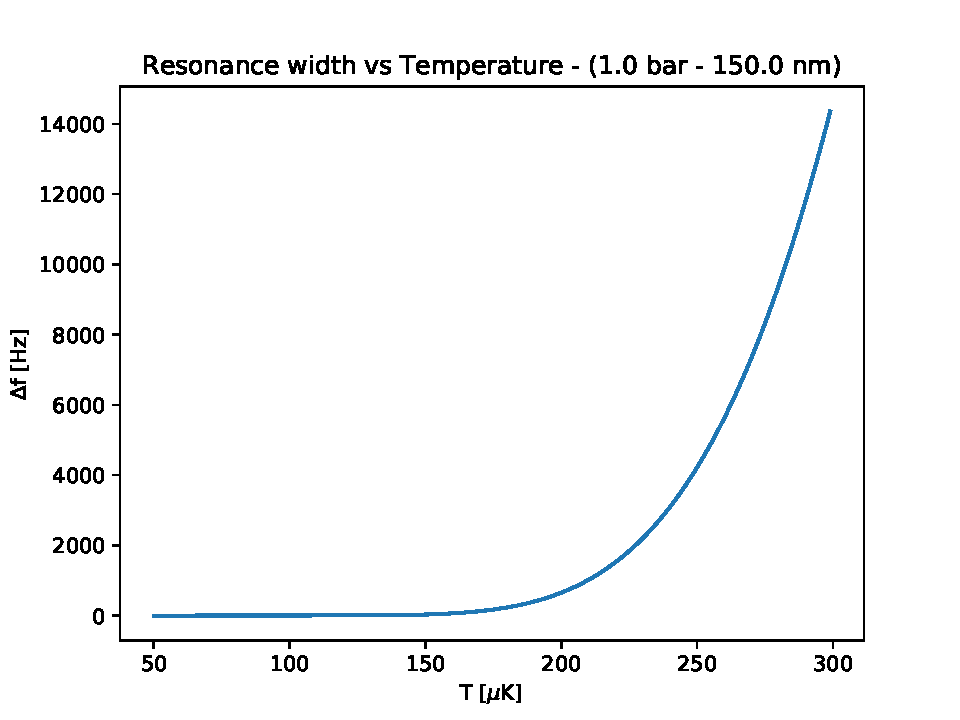
\includegraphics[width=0.69\textwidth]{W_vs_T}
    \caption{Resonance frequency width dependence on temperature for a nano-wire.}
    \label{fig:WvsT}
  \end{center}
\end{figure}

\begin{equation}
T = - \frac{\Delta}{k_B \ln \left( \Delta f \frac{2 \pi \rho d}{p_F^2 v_F N(0)} \right)}
\end{equation}

The increase of resonance width $\Delta (\Delta f)$ in response of an energy deposition $\Delta Q$ is linearly proportional, as shown in figure~\ref{fig:DeltaDeltaWvsDE}.
The constant of proportionality is inversely proportional to the base temperature, so the other way around, in terms of energy deposition
\begin{equation}
  \Delta Q = \alpha(T_0) \Delta (\Delta f), \alpha \propto T_0
\end{equation}

\begin{figure}[!ht]
  \begin{center}
  \begin{tabular}{cc}
    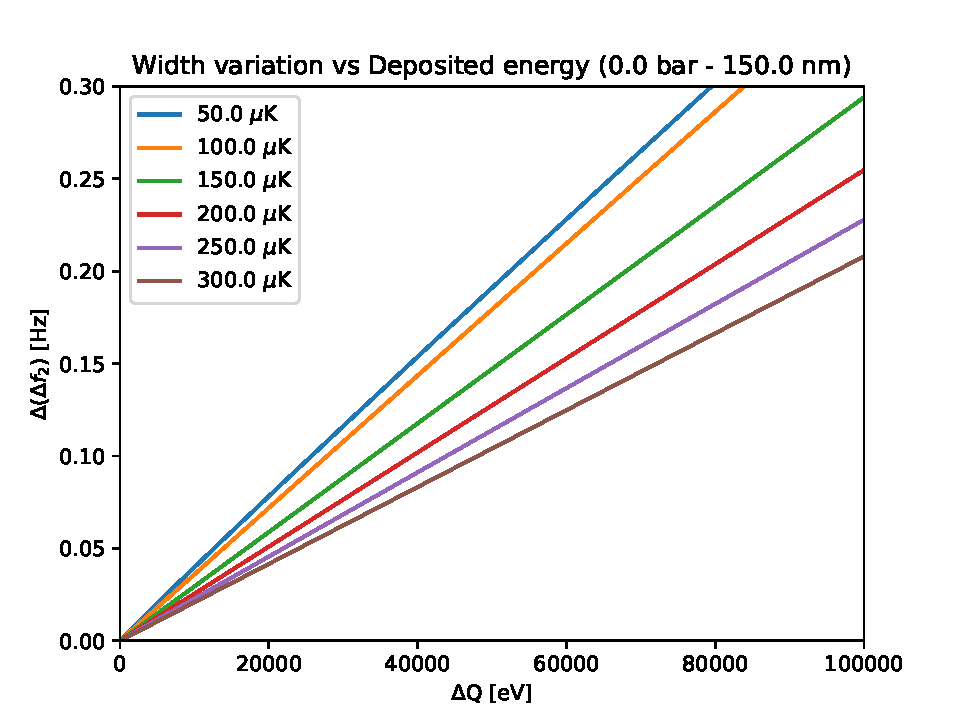
\includegraphics[width=0.49\textwidth]{DeltaDeltaW_vs_DE-0bar}  &
    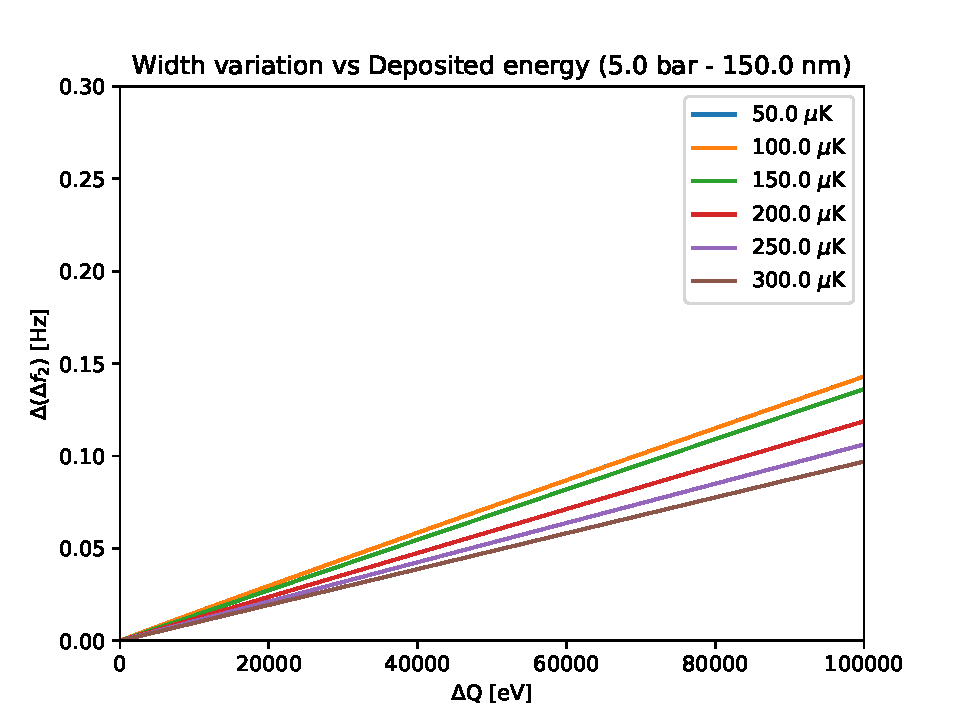
\includegraphics[width=0.49\textwidth]{DeltaDeltaW_vs_DE-5bar}  \\
    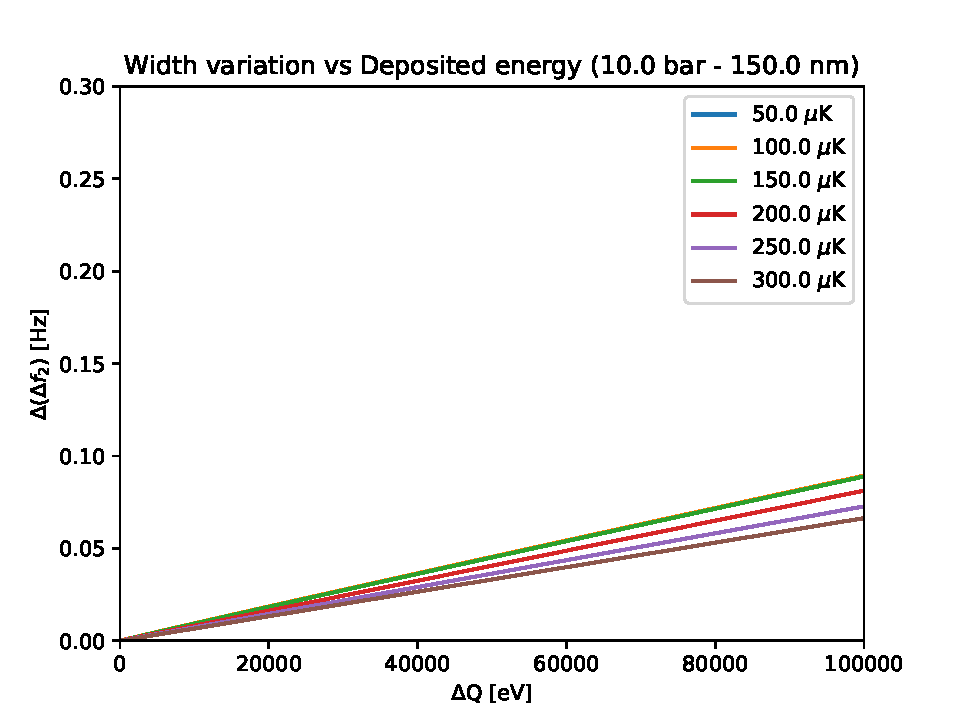
\includegraphics[width=0.49\textwidth]{DeltaDeltaW_vs_DE-10bar} &
    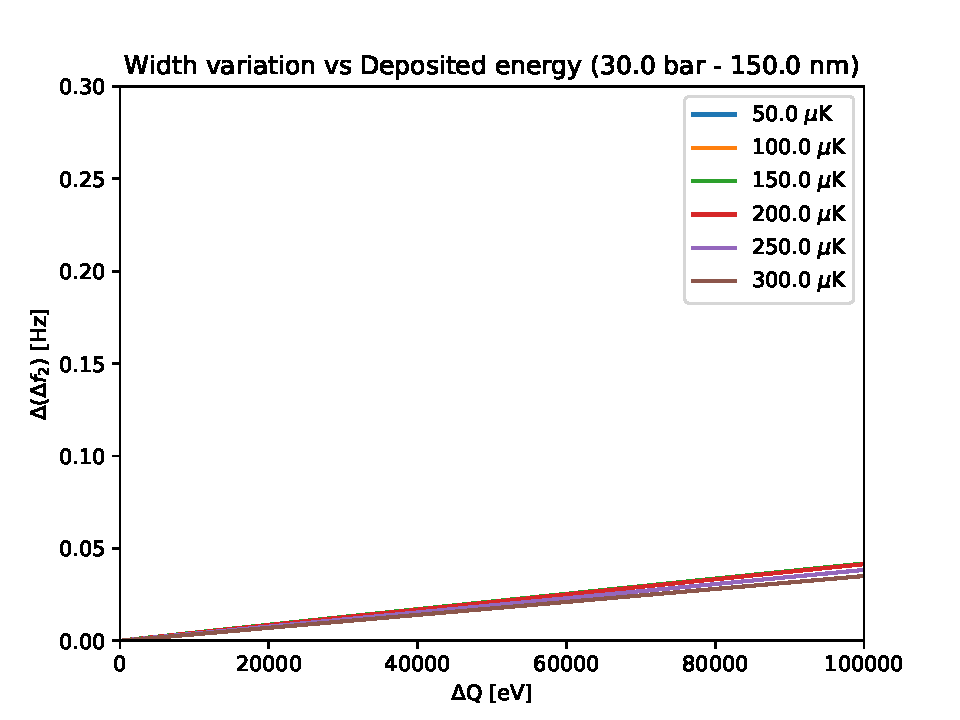
\includegraphics[width=0.49\textwidth]{DeltaDeltaW_vs_DE-30bar}
  \end{tabular}
  \end{center}
  \caption{$\Delta(\Delta f)$ vs $\Delta Q$ for several $T_0$ in the range 50--300\,$\mu$K for pressures of 0\,bar (top-left), 5\,bar (top-right), 10\,bar (bottom-left), 30\,bar (bottom-right).}
  \label{fig:DeltaDeltaWvsDE}
\end{figure}

The increase of resonance width $\Delta (\Delta f)$ can be measured from fitting each bolometric recorded event, e.g. in figure~\ref{fig:winkelmann} from~\cite{winkelmann},
\begin{figure}[!ht]
  \begin{center}
    \begin{tabular}{cc}
    \includegraphics[width=0.42\textwidth]{winkelmann} &
    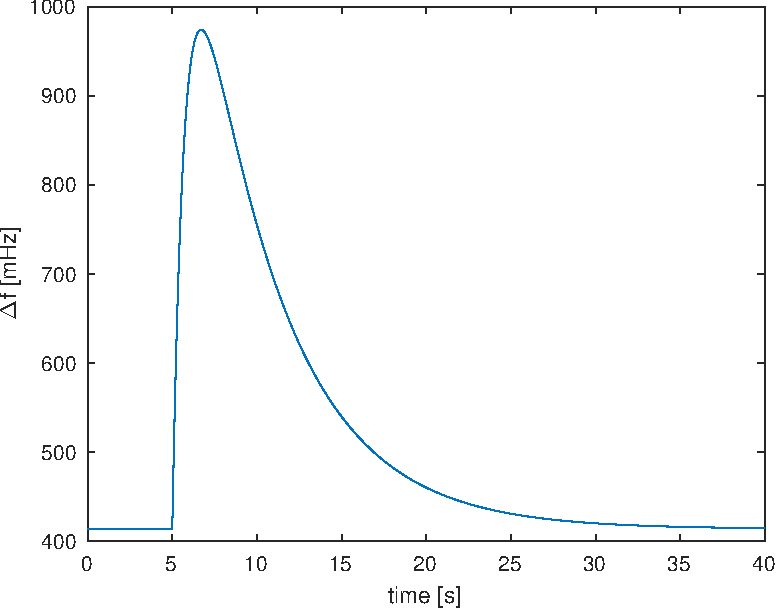
\includegraphics[width=0.49\textwidth]{winkelmann_fit.pdf}
    \label{fig:winkelmann}
    \end{tabular}
  \end{center}
 \caption{Example of an energy deposition event for a 4.5\,$\mu$m wire in a volume of 0.14\,cm$^3$ of He-3. H in the paper's notation is proportional to $\Delta (\Delta f)$ with respect to a base width~\cite{winkelmann} (\textit{left}); fit function as in eq.~\ref{fit} (\textit{right}) with $\tau_b$=5\,s and $\tau_w$=0.77\,s;.}
\end{figure}
using the function

\begin{equation}
  \Delta f = \Delta f_\mathrm{base} + \Delta (\Delta f) {\left( \frac{\tau_b}{\tau_w} \right)}^{\tau_w/(\tau_b-\tau_w)} \frac{\tau_b}{\tau_b - \tau_w} \left( e^{-t/\tau_b} - e^{-t/\tau_w} \right)
\label{fit}
\end{equation}

in order to extract the maximum variation $\Delta (\Delta f)$, where $\Delta f_\mathrm{base}$ is the base width at the base temperature of the helium, $\tau_w$ is the response time of the oscillating wire
\begin{equation}
  \tau_w \simeq \frac{1}{\pi \Delta f} = \mathrm{const}
\end{equation}
and $\tau_b$ is the decay constant, proportional to the Kapitza resistance (the thermal boundary resistance limiting the heat conduction between the solid metal and the liquid helium)
\begin{equation}
  \tau_b = R_K(T) C_V
\end{equation}

Considering that there are three main variables, base temperature, pressure of the helium, wire diameter (considering fixed the wire material and the helium volume), all with an interplay between each other, we can at least extract few conclusions:
\begin{itemize}
  \item For small wires there is an higher amplitude of the width response $\Delta (\Delta f)$
  \item For low temperatures there is an higher amplitude of the width response $\Delta (\Delta f)$
  \item For high pressures there is a lower width response for a certain energy deposition
  \item The response time of the oscillating wire is faster for high temperatures 
  \item The decay time of the oscillating wire is faster for high temperatures (low Kapitza resistance), so low temperatures might cause some pile-up of events

\end{itemize}

Open questions:
\begin{itemize}

  \item What is the minimum width variation we can measure, hence the threshold of the energy deposition? 
  \item Which is the resolution in the resonance width variation (aka temperature variation), hence the resolution of the energy deposition?

\end{itemize}


% ============================================

\section{Errors}

We assume that the main uncertainty comes from the variation of resonance width $\Delta f$ of the wire, the error on the energy deposition would be

\begin{equation}
  \sigma_{\Delta Q}  \simeq \frac{\partial \Delta Q}{\partial(\Delta(\Delta f))} \sigma_{\Delta (\Delta f)}
\end{equation}

which ultimately comes to the uncertainty in the fitting procedure and the uncertainty in the fast width measurement.

% ============================================
\pagebreak
\newpage

\begin{thebibliography}{9}

\bibitem{vollhardt} Vollhardt, D., Wolfle, P., The Superfluid Phases of Helium 3 (1990)
\bibitem{lawson} Lawson C., thesis (2014)
\bibitem{winkelmann} Winkelmann et al, Bolometric calibration of a superfluid 3He detector for Dark Matter search: Direct measurement of the scintillated energy fraction for
neutron, electron and muon events (2007)

\end{thebibliography}

\end{document}
